\begin{figure}[h]
\centering
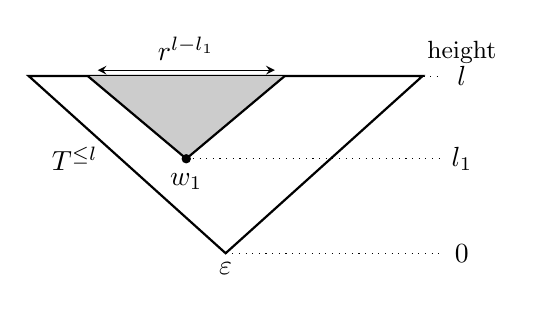
\begin{tikzpicture}[x=2.5cm, y=1.5cm]
    % رسم مثلث اصلی (درخت T^l)
    \draw[thick] (0,0) -- (-1,1.5) -- (1,1.5) -- cycle;
    
    % رسم ناحیه هاشور خورده (زیردرخت غلبه شده توسط w1)
    \fill[gray!40] (-0.2,0.8) -- (-0.7,1.5) -- (0.3,1.5) -- cycle;
    \draw[thick] (-0.2,0.8) -- (-0.7,1.5);
    \draw[thick] (-0.2,0.8) -- (0.3,1.5);
    
    % فلش دو سر برای نشان دادن تعداد برگ‌ها (r^{l-l1})
    \draw[<->, >=stealth] (-0.65,1.55) -- node[above] {$r^{l-l_1}$} (0.25,1.55);
    
    % برچسب‌های نقاط و سطوح
    \node[circle, fill, inner sep=1.2pt, label=below:$w_1$] at (-0.2,0.8) {};
    \node[below] at (0,0) {$\varepsilon$};
    \node[left] at (-0.6,0.8) {$T^{\le l}$};
    
    % محور ارتفاع در سمت راست
    \node at (1.2, 1.7) {\small height};
    \node at (1.2, 1.5) {$l$};
    \node at (1.2, 0.8) {$l_1$};
    \node at (1.2, 0) {$0$};
    
    % خطوط راهنمای افقی (نقطه چین) برای ارتفاع
    \draw[dotted] (0.6,1.5) -- (1.1,1.5);
    \draw[dotted] (-0.2,0.8) -- (1.1,0.8);
    \draw[dotted] (0,0) -- (1.1,0);

\end{tikzpicture}
\caption{}
\end{figure}